\section{Conceptual Design}

\subsection{Variations to the Requirement Analysis}
we changed some parts of the last homework to make it better as follows:

Owner, Inventory, Sales are removed and other entities which are mentioned in the following tables have been added to our schema. 
A modern database is needed which makes a bookshop able to sell its books through an online platform. This system has customers and admins as users. Customers login with their email and password and can take a look at the items of the shop and buy them or chat with the support department. Admins can login with their username and password and modify the books in the website or answer the customers(based on their role in the system). Every book in the system has its own publisher and writer and the copies of these books are held in the warehouses. After a purchase is made , Items are packed into a package and they are sent to the customer using different shipping companies in maximum 3 working days.
\subsection{Entity-Relationship Schema}
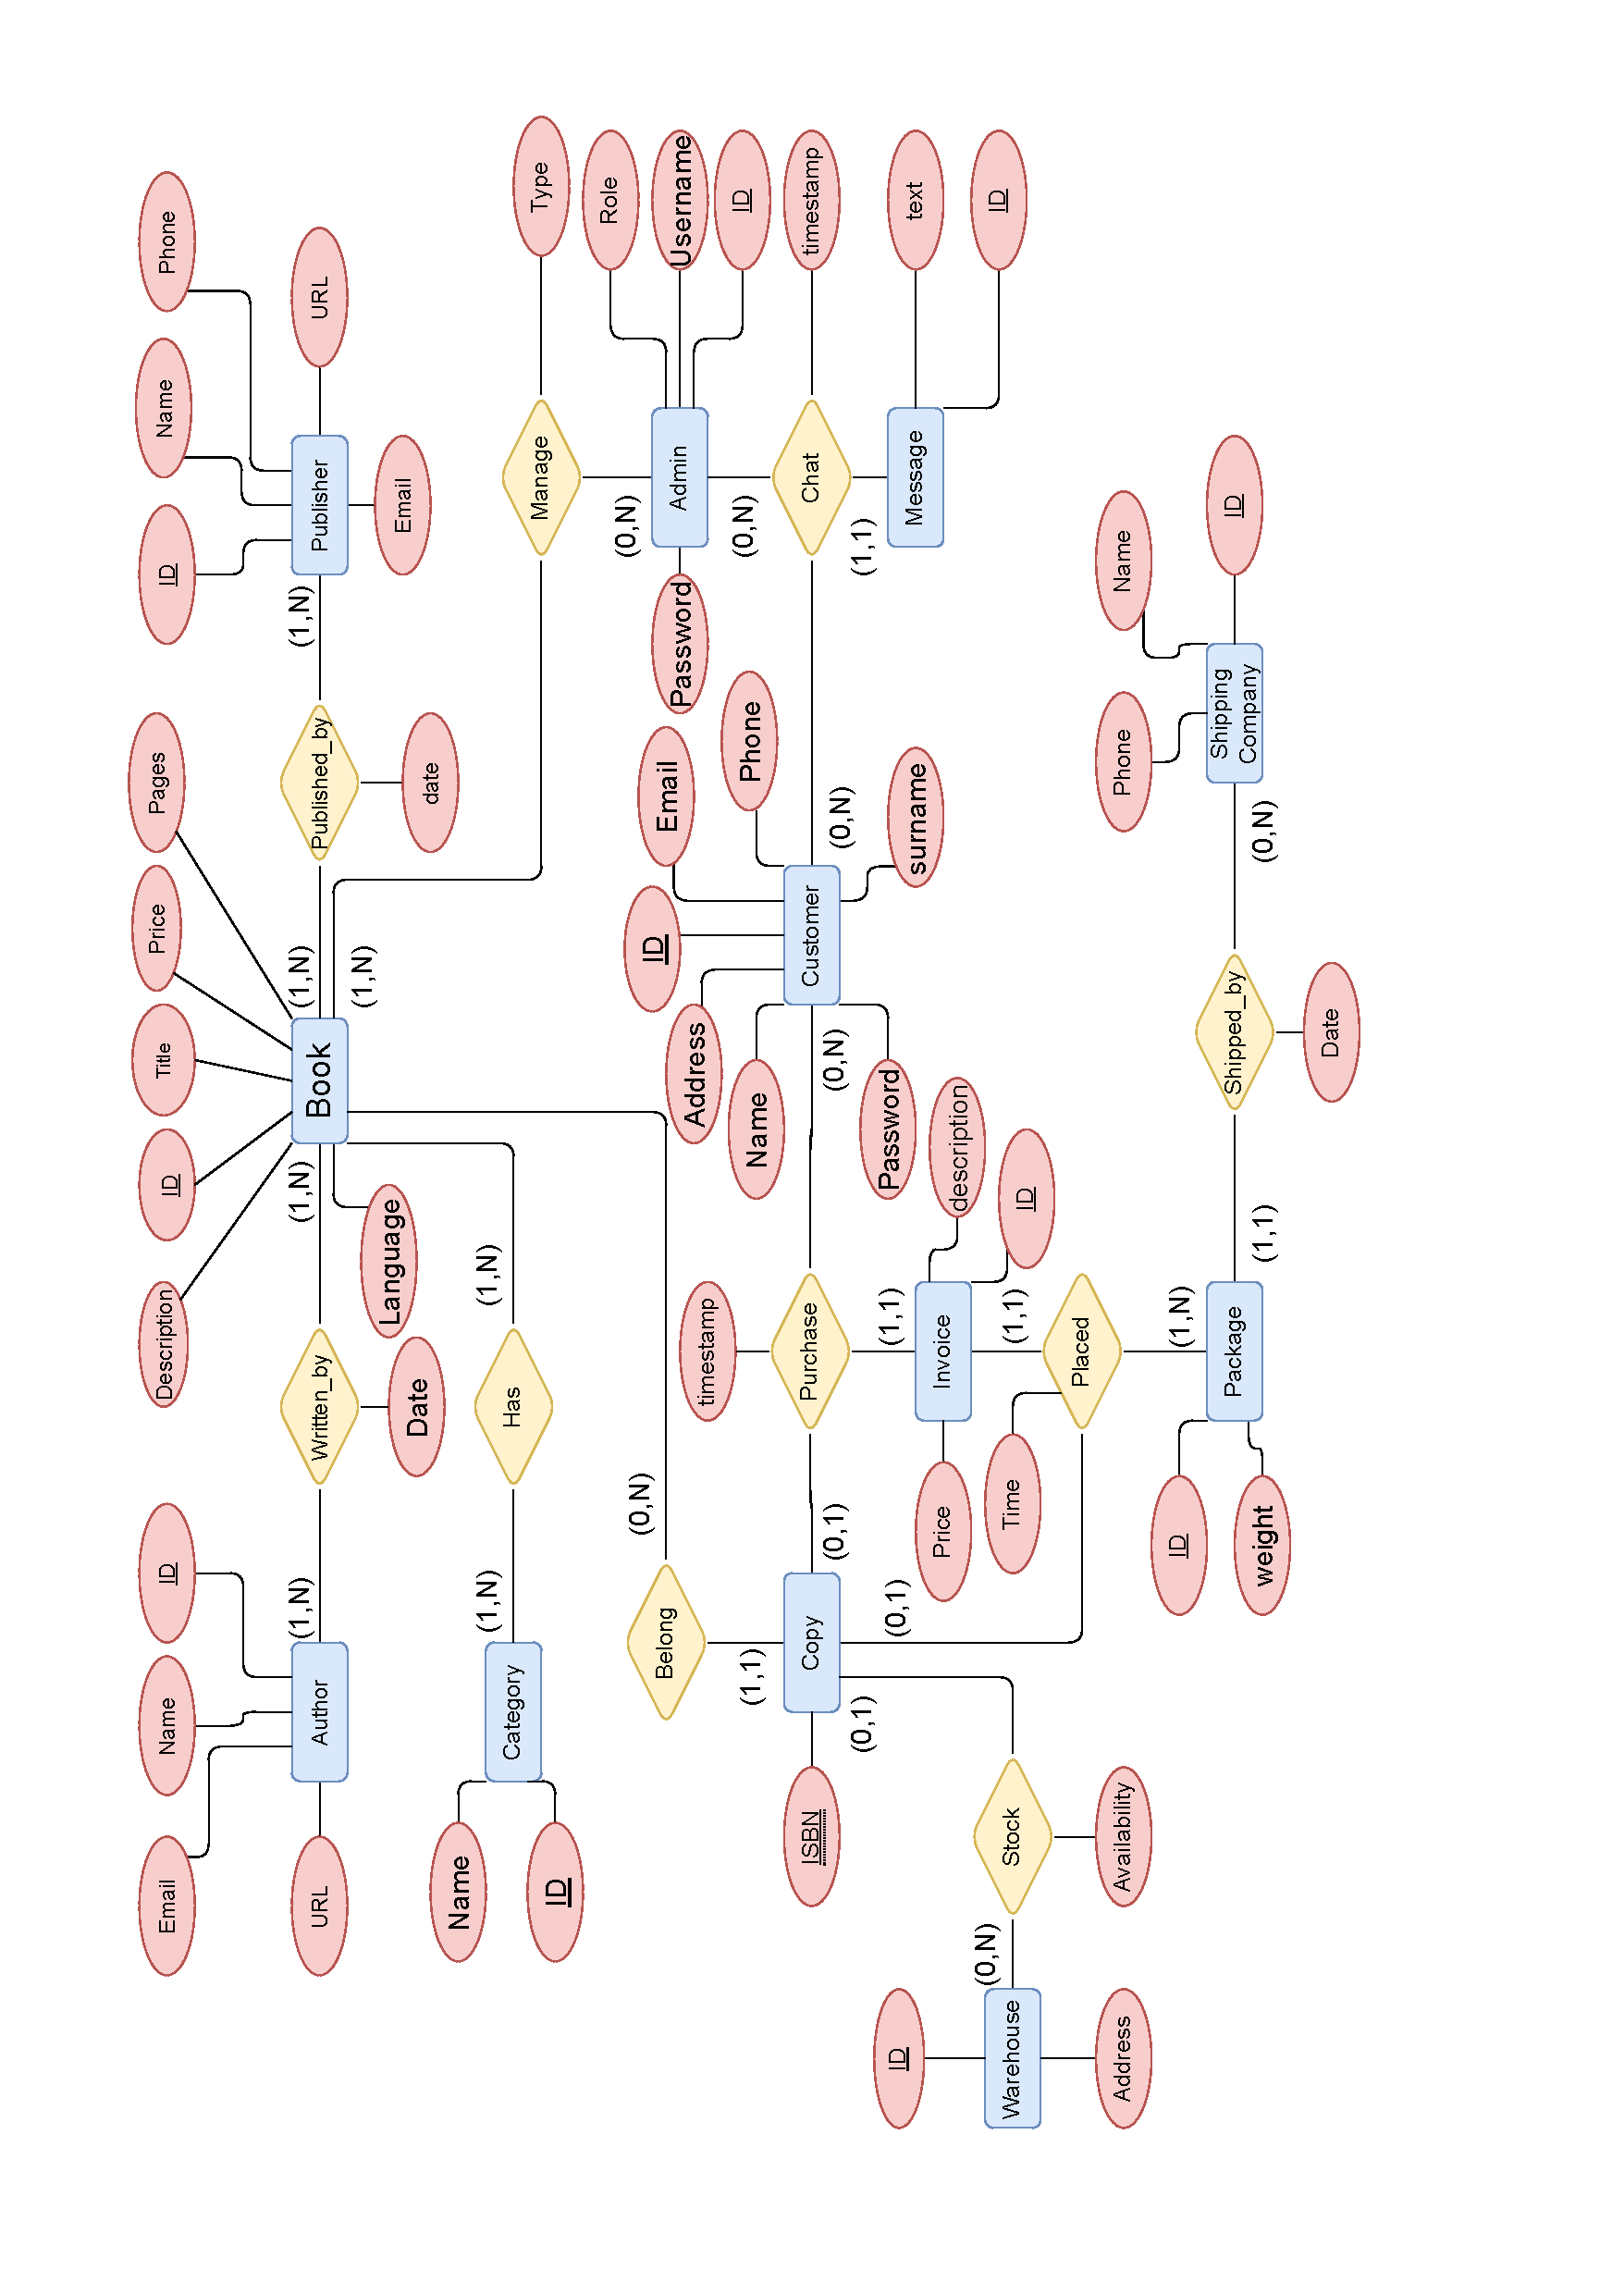
\includepdf[scale=0.9]{sections/ERschema.pdf}
\subsection{Data Dictionary}

\subsubsection{Entities Table}
\begin{longtable}{|p{.20\columnwidth}|p{.20\columnwidth} |p{.30\columnwidth}|p{.25\columnwidth} |} 
\hline
\textbf{Entity} & \textbf{Description} & \textbf{Attributes} & \textbf{Identifier}  \\\hline


Book & the Catalogue of the Books in our website which shows the book and its description to the customers & \begin{itemize}
        \vspace{-1em}
        \item ID: Book identifier (serial)
         \item Description: a brief information about the book (text)
        \item Title: title of the book(text)
        \item price: the cost of the book (float)
        \item pages: the number of pages of the book (integer)
        \item Language: the language of the book in which the book is written to



    \end{itemize}
 &  ID\\\hline
 
Author & the author of the book who has written it & \begin{itemize}
        \vspace{-1em}
        \item ID: author identifier (serial)
        \item Name: Full name of the author(text)
        \item URL: the link to the personal webpage of the author(text)
        \item Email: email address of the author(text)
    \end{itemize}
 &  ID \\\hline
 
 
  Copy & the physical book which is held in the warehouse and will be delivered to the customer & \begin{itemize}
        \vspace{-1em}
        \item ISBN: The International Standard Book Number is a numeric commercial book identifier that is intended to be unique. (serial)
        
    \end{itemize}
 &  ISBN \\\hline
 
 
   Publisher & The company who published the book & \begin{itemize}
        \vspace{-1em}
        \item ID: publisher identifier (serial)
        \item Name: the name of the publishing company (text)
        \item URL: publisher website link (text)
        \item Phone: the phone number to access the publisher (integer)
        \item Email: the publisher email (text)
    \end{itemize}
 &  ID \\\hline

  Customer & the customer of the bookshop who logs in with their username and password and purchase the book, they can also chat with admins & \begin{itemize}
        \vspace{-1em}
        \item ID: identifier of the customer (serial)
        \item Name: first name of the customer (text)
        \item Address: the address of the customer which the books will be delivered to (text)
        \item Email: email of the customer which is used also to log in
        \item Phone: the phone number of the customer (integer)
        \item surname: the last name of the customer (text)
        \item Password: the password which is used to login to the system (text)
    \end{itemize}
 &  ID \\\hline
 
   Admin & the admin of the system who logs in with username and password and can edit the information of each book,add or delete the books and chat with customers & \begin{itemize}
        \vspace{-1em}
        \item ID: identifier of the admin (serial)
        \item Role: the role of the admin in the system,they can be in Support department or the ones who add or delete the books, change prices or write description of the books(Manage department) (text)
        \item username: the username to login(text)
        \item password: the pass word to login(text)
    \end{itemize}
 &  ID \\\hline
 
   Message & the messages in the chat between customer and admins & \begin{itemize}
        \vspace{-1em}
        \item ID: identifier of the message(serial)
        \item text: the text of the message written by admin and customer (text)
    \end{itemize}
 &  ID \\\hline
 
   Invoice & the invoice or bill created after the customer purchase containing the information about order  & \begin{itemize}
        \vspace{-1em}
        \item ID: identifier of the invoice (serial)
        \item Price: the price of the purchase
        \item description: the notes about the purchase (text)
    \end{itemize}
 &  ID \\\hline
 
   Warehouse & the warehouse of the shop which stores the physical books & \begin{itemize}
        \vspace{-1em}
        \item ID: identifier of the warehouse (serial)
        \item address: the address of where the warehouse is located (text)
    \end{itemize}
 &  ID \\\hline
 
   Category & the genre of the books & \begin{itemize}
        \vspace{-1em}
        \item ID: identifier of the category(serial)
        \item Name: the name of the category (text)
    \end{itemize}
 &  ID \\\hline
 
   Package & the package containing of a customer purchase and will be delivered & \begin{itemize}
        \vspace{-1em}
        \item ID: identifier of the package (serial)
        \item weight: the weight of the package to calculate the cost of delivery (float)
    \end{itemize}
 &  ID \\\hline
 
 
    shipping company & the company which collect the packages and delivers it to customer & \begin{itemize}
        \vspace{-1em}
        \item ID: identifier of the company
        \item Name: name of the company
        \item Phone: phone number of the company
    \end{itemize}
 &  ID \\\hline
 
\end{longtable}


\subsubsection{Relationships Table}
\begin{longtable}{|p{.20\columnwidth}|p{.20\columnwidth} |p{.30\columnwidth}|p{.25\columnwidth} |} 
\hline
\textbf{Relationship} & \textbf{Description} & \textbf{Component Entities} & \textbf{Attributes} \\\hline


Written\_by & it associates a book to an author and identifies the author who has written the book & \begin{itemize}
        \vspace{-1em}
        \item Author (1,N): an author has written several books and at least one
        \item Book (1, N)
    \end{itemize}
 & date: the date in which the book was written by author \\\hline
 
 Published\by & it associates a book to a publisher and identifies which publisher published the book & \begin{itemize}
        \vspace{-1em}
        \item Book (1, N)
        \item Publisher (1,N) 
    \end{itemize}
 &  date: the date in which the book was published by publisher \\\hline
 
  Has & it associates a Book to Categories and identifies the categorie(s) of a book & \begin{itemize}
        \vspace{-1em}
        \item Book (1, N)
        \item Category (1, N)
    \end{itemize}
 &   \\\hline
 
  Manage & it relates an admin to a book and shows which admin modified the book & \begin{itemize}
        \vspace{-1em}
        \item Book (1, N)
        \item Admin (0,N): multiple admins can manage a book
    \end{itemize}
 &  Type: it shows the type of the management,it could be add,remove,modify \\\hline
 
  Chat & it associates a customer to an admin and the message which has been used to chat between them & \begin{itemize}
        \vspace{-1em}
        \item Admin (0, N)
        \item Customer (0, N)
        \item Message (1, 1): a message is associated between one and only one customer and admin
    \end{itemize}
 &  timestamp: the time of the chat took place at \\\hline
 
  Belong & it associates a copy to a book & \begin{itemize}
        \vspace{-1em}
        \item Book (0, N)
        \item Copy (1, 1): a copy can belong to one and only one book
    \end{itemize}
 &   \\\hline
 
  Purchase & it associates a customer to a copy and the invoice created for this order & \begin{itemize}
        \vspace{-1em}
        \item Customer (0, N)
        \item Copy (0, 1): a copy can be purchased only by one customer
        \item Invoice (1, 1)
    \end{itemize}
 &  timestamp: the time in which the purchase took place at \\\hline
 
  Stock & it associates a Copy to a warehouse and identifies a copy is held in which warehouse & \begin{itemize}
        \vspace{-1em}
        \item Copy (0, 1)
        \item warehouse (0, N)
    \end{itemize}
 &  availability: a boolean which tells us if a book is available or not \\\hline
 
  Placed & it associates a copy to an invoice (which was made through the purchase) to a packages,it shows which packages contains the copies bought by the customer & \begin{itemize}
        \vspace{-1em}
        \item invoice (1, 1)
        \item Copy (0, 1)
        \item Package (1, 1)
        

    \end{itemize}
 &  Time: time of the package was packed  \\\hline
 
  Shipped\_by & it relates a package to a shipping company and shows the package was shipped by which company & \begin{itemize}
        \vspace{-1em}
        \item Package (1, 1)
        \item Shipping Company (0, N)
    \end{itemize}
 &  date: date of the shipping \\\hline

\end{longtable}

\subsection{External Constraints}
\begin{itemize}
        
        \item The admin can changes the book(add,delete,change price,change description) depending on his Role
        \item The customer can only purchase the book which is available in the warehouses.
        \item The package should be shipped by the shipper due to time limit that is announced in the website(for example it says in 3 working days it will be delivered)
        \item The customer should only chat to the admin whose Role is Support.
    \end{itemize}
    
\subsection{Functional Requirements Satisfaction Check}
The system must allow:
\begin{itemize}
\item \textbf{To store customer information}
\end{itemize}
All the information about the customer are stored as attributes. There are attributes like:
\begin{enumerate}
\item Address
\item Name
\item ID
\item E-mail
\item Phone
\end{enumerate} 
Address is a necessary information about the functionality of the bookstore since the shipper must know where he needs to send the products that are bought by the customer. 

\begin{itemize}
\item \textbf{To store information about the books}
\end{itemize}
Each book will have its own details. The attributes of this entity are: 
\begin{enumerate}
\item ID
\item Title
\item Description
\item Language
\item Price
\item Pages
\end{enumerate}
They will hold all the necessary information about this entity. 

\begin{itemize}
\item \textbf{To manage multiple purchases by each customer} 
\end{itemize}
The "Copy" entity and its 'Purchase' relationship with "Customer" and the cardinality of these relations make it possible that a customer can buy multiple copies of the same book or different books.

\begin{itemize}
\item \textbf{To store information about the purchases that are done}
\end{itemize}
The ternary 'Purchase' relationship between 'Customer', 'Copy', 'Invoice' ensures that every purchase will be stored in the database together with the timestamp which will hold information about the time when a customer has purchased a copy of a book

\begin{itemize}
\item \textbf{The Ability to add new books on the system of the bookshop and modifies data related to existing books}
\end{itemize}
The menage relationship between the admin and the book entity make it possible for admin to add, delete, update the data that is stored for a book.

\begin{itemize}
\item \textbf{Admin and customers to log in}
\end{itemize}
Both entities 'Admin' and 'Customer' have attributes which will help them to log into the application. Admin will log in using username and password. The customers will log in using email and their passwords.    

\begin{itemize}
\item \textbf{Has to store information about the packages that are created and the company that will ship a package }
\end{itemize}
'Package' entity and '\texttt{Shipped\_by}' relationship ensures that this requirement will be satisfied. The 'Package' will store information about all the copies that are purchased by a customer in the same timestamp. \texttt{Shipped\_by} on the other hand relates the package with the company that will deliver it. 

\begin{itemize}
\item \textbf{The database will store information about different authors and publisher}
\end{itemize}
Author and Publisher are two entities in our database that will contain the required data and meet this criteria. The unique ID assigned to each author and publisher will serve as their identify. In addition, there will be more characteristics concerning other information.